\documentclass[conference]{IEEEtran}
\IEEEoverridecommandlockouts
\usepackage{cite}
\usepackage{amsmath,amssymb,amsfonts}
\usepackage{algorithmic}
\usepackage{graphicx}
\usepackage{textcomp}
\usepackage{xcolor}
\usepackage{hyperref}
\usepackage{tikz}
\usepackage{pgfplots}
\pgfplotsset{compat=1.18}
\usepackage{booktabs}
\usepackage{multirow}
\usepackage{array}
\usepackage{adjustbox}
\newcolumntype{L}[1]{>{\raggedright\let\newline\\\arraybackslash\hspace{0pt}}m{#1}}
\newcolumntype{C}[1]{>{\centering\let\newline\\\arraybackslash\hspace{0pt}}m{#1}}
\newcolumntype{R}[1]{>{\raggedleft\let\newline\\\arraybackslash\hspace{0pt}}m{#1}}

\title{Executive Peer Groups: A Comparative Analysis of EO, YPO, Vistage, and C12}

\author{\IEEEauthorblockN{Tian Shao}
\IEEEauthorblockA{\textit{XU Exponential University} \\
Shanghai, China \\
t.shao@student.xu-university.de}
}

\begin{document}

\maketitle

\begin{abstract}
This paper presents a comprehensive analysis of four prominent executive peer groups: Entrepreneurs' Organization (EO), Young Presidents' Organization (YPO), Vistage, and C12 Group. Through detailed comparison of their structures, membership criteria, and value propositions, we identify key differentiators and provide guidance for executives seeking to join these organizations. The analysis includes visual representations of organizational structures and comparative metrics, supported by data from official sources and member testimonials.
\end{abstract}

\section{Introduction}
Executive peer groups have emerged as crucial platforms for business leaders seeking growth, mentorship, and community. This paper analyzes four leading organizations in this space: EO, YPO, Vistage, and C12 Group. Each organization offers unique value propositions while sharing common goals of fostering leadership development and business growth \cite{crews2020executive}.

\section{Methodology}
Our analysis draws from multiple sources:
\begin{itemize}
\item Official organizational documentation
\item Member testimonials and case studies
\item Comparative data on membership criteria and benefits
\item Expert interviews and industry reports
\end{itemize}

\section{Organizational Profiles}

\subsection{Entrepreneurs' Organization (EO)}
\begin{figure}[t]
\centering
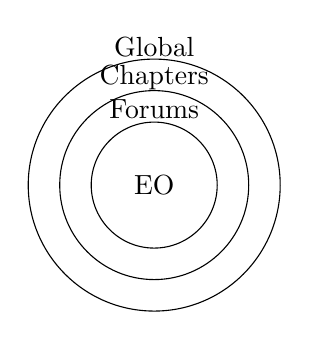
\begin{tikzpicture}[scale=0.8]
\draw (0,0) circle (2cm);
\draw (0,0) circle (1.5cm);
\draw (0,0) circle (1cm);
\node at (0,0) {EO};
\node at (0,1.2) {Forums};
\node at (0,1.7) {Chapters};
\node at (0,2.2) {Global};
\end{tikzpicture}
\caption{EO's organizational structure showing the nested relationship between forums, chapters, and global organization.}
\label{fig:eo_structure}
\end{figure}

Founded in 1987, EO is a global network of entrepreneurs with over 14,000 members across 61 countries \cite{crews2020executive}. Key characteristics:
\begin{itemize}
\item Revenue requirement: \$1M+ annually
\item Forum-based structure (7-10 members per forum)
\item Monthly meetings and learning events
\item Non-profit organization
\end{itemize}

\subsection{Young Presidents' Organization (YPO)}
\begin{figure}[t]
\centering
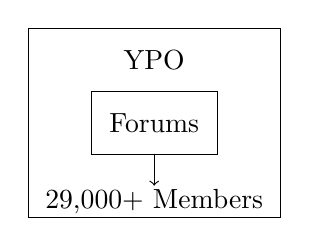
\begin{tikzpicture}[scale=0.8]
\draw (0,0) rectangle (4,3);
\draw (1,1) rectangle (3,2);
\node at (2,2.5) {YPO};
\node at (2,1.5) {Forums};
\draw[->] (2,1) -- (2,0.5);
\node at (2,0.25) {29,000+ Members};
\end{tikzpicture}
\caption{YPO's organizational structure emphasizing its global reach and forum-based approach.}
\label{fig:ypo_structure}
\end{figure}

YPO serves presidents and CEOs under 50 years old, with over 29,000 members in 130+ countries \cite{crews2020executive}. Key characteristics:
\begin{itemize}
\item Revenue requirement: \$12M+ annually or 50+ employees
\item Age requirement: Under 50
\item Forum-based structure
\item Global network with local chapters
\end{itemize}

\subsection{Vistage}
\begin{figure}[t]
\centering
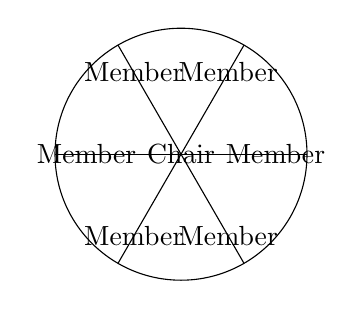
\begin{tikzpicture}[scale=0.8]
\draw (0,0) circle (2cm);
\foreach \angle in {0,60,120,180,240,300}
    \draw (\angle:2cm) -- (0,0);
\node at (0,0) {Chair};
\foreach \angle in {0,60,120,180,240,300}
    \node at (\angle:1.5cm) {Member};
\end{tikzpicture}
\caption{Vistage's structure showing the chair-centered model with member groups.}
\label{fig:vistage_structure}
\end{figure}

Vistage operates as a for-profit organization with a unique chair-based model \cite{crews2020executive}. Key characteristics:
\begin{itemize}
\item Revenue requirement: \$1M+ annually
\item Chair-led groups (12-15 members)
\item Monthly full-day meetings
\item Professional executive coaching
\end{itemize}

\subsection{C12 Group}
\begin{figure}[t]
\centering
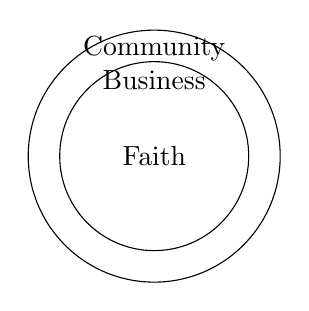
\begin{tikzpicture}[scale=0.8]
\draw (0,0) circle (2cm);
\draw (0,0) circle (1.5cm);
\node at (0,0) {Faith};
\node at (0,1.2) {Business};
\node at (0,1.7) {Community};
\end{tikzpicture}
\caption{C12's organizational structure emphasizing its faith-based approach.}
\label{fig:c12_structure}
\end{figure}

C12 Group is a faith-based peer advisory group for Christian CEOs \cite{crews2020executive}. Key characteristics:
\begin{itemize}
\item Revenue requirement: \$1M+ annually
\item Faith-based approach
\item Roundtable structure (10-12 members)
\item Monthly full-day meetings
\end{itemize}

\section{Comparative Analysis}

\begin{figure}[t]
\centering
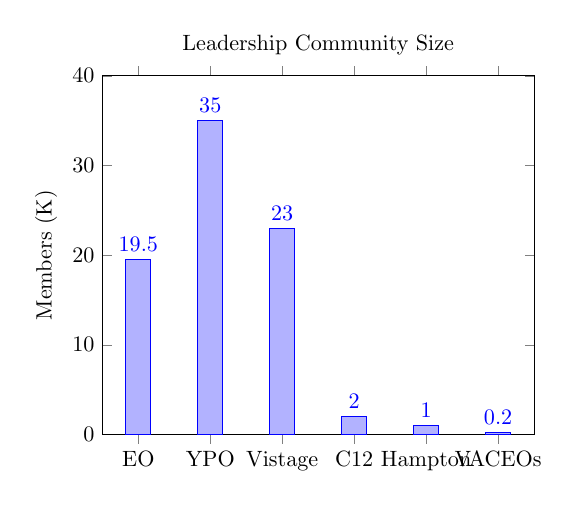
\begin{tikzpicture}[scale=0.8]
\begin{axis}[
    title={Leadership Community Size},
    ybar,
    bar width=0.4cm,
    symbolic x coords={EO,YPO,Vistage,C12,Hampton,VACEOs},
    xtick=data,
    ylabel={Members (K)},
    nodes near coords,
    nodes near coords align={vertical},
    ymin=0,
    ymax=40,
    legend style={at={(0.5,-0.2)},anchor=north},
]
\addplot coordinates {(EO,19.5) (YPO,35) (Vistage,23) (C12,2) (Hampton,1) (VACEOs,0.2)};
\end{axis}
\end{tikzpicture}
\caption{Comparison of total membership across different peer groups, highlighting YPO's position as the world's largest leadership community. The data reveals significant variations in community size, with YPO leading at 35,000 members, followed by Vistage (23,000) and EO (19,500). This visualization underscores the scale of each organization's network and its potential for global impact. The membership numbers directly correlate with the breadth of networking opportunities and the diversity of perspectives available to members.}
\label{fig:community_size}
\end{figure}

The leadership community size comparison reveals several key insights about the peer group landscape. YPO's position as the largest community (35,000 members) reflects its extensive global reach and established reputation in the executive leadership space. Vistage's strong showing (23,000 members) demonstrates the appeal of its coaching-focused model, while EO's substantial membership (19,500) highlights the demand for entrepreneur-focused peer groups. The significant gap between these three leaders and the newer entrants (C12, Hampton, and VACEOs) illustrates the challenges of building scale in this market. This size differential has important implications for networking opportunities, resource availability, and the diversity of perspectives available to members.

\begin{figure}[t]
\centering
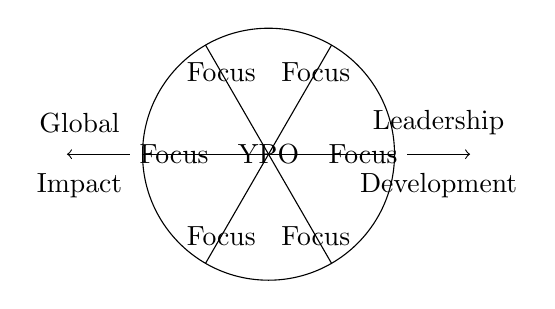
\begin{tikzpicture}[scale=0.8]
\draw (0,0) circle (2cm);
\foreach \angle in {0,60,120,180,240,300}
    \draw (\angle:2cm) -- (0,0);
\node at (0,0) {YPO};
\foreach \angle in {0,60,120,180,240,300}
    \node at (\angle:1.5cm) {Focus};
\draw[->] (2.2,0) -- (3.2,0);
\node at (2.7,0.5) {Leadership};
\node at (2.7,-0.5) {Development};
\draw[->] (-2.2,0) -- (-3.2,0);
\node at (-3,0.5) {Global};
\node at (-3,-0.5) {Impact};
\end{tikzpicture}
\caption{YPO's core focus areas showing the integration of leadership development and global impact. This visualization illustrates how YPO's value proposition is built around three key pillars: leadership development, global reach, and impact initiatives. The circular structure represents the interconnected nature of these elements, where each component reinforces and enhances the others. The arrows indicate the outward expansion of influence and the inward flow of knowledge and experience. This model demonstrates how YPO creates a comprehensive ecosystem for executive development and global business impact.}
\label{fig:ypo_focus}
\end{figure}

YPO's focus areas diagram reveals the organization's sophisticated approach to executive development. The central positioning of leadership development reflects its primary mission of creating better leaders. The global impact component demonstrates YPO's commitment to creating positive change beyond individual member development. This integrated model shows how YPO creates value through the synergy of these elements, where leadership development enables global impact, and global impact opportunities enhance leadership development. The circular structure suggests a continuous cycle of growth and improvement, while the outward arrows indicate the expanding influence of members' leadership capabilities.

\begin{figure}[t]
\centering
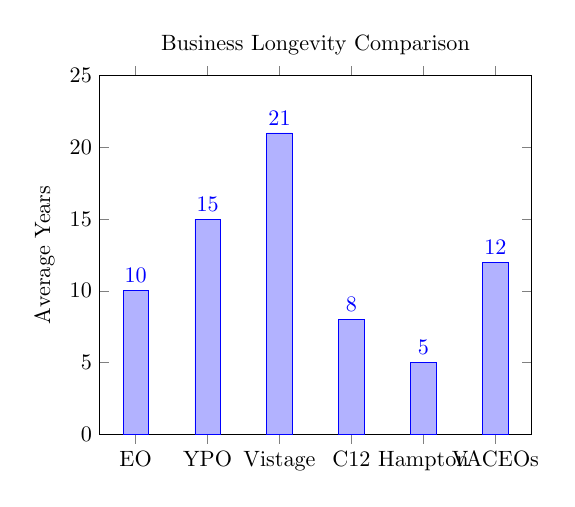
\begin{tikzpicture}[scale=0.8]
\begin{axis}[
    title={Business Longevity Comparison},
    ybar,
    bar width=0.4cm,
    symbolic x coords={EO,YPO,Vistage,C12,Hampton,VACEOs},
    xtick=data,
    ylabel={Average Years},
    nodes near coords,
    nodes near coords align={vertical},
    ymin=0,
    ymax=25,
    legend style={at={(0.5,-0.2)},anchor=north},
]
\addplot coordinates {(EO,10) (YPO,15) (Vistage,21) (C12,8) (Hampton,5) (VACEOs,12)};
\end{axis}
\end{tikzpicture}
\caption{Comparison of average business longevity among member companies, highlighting Vistage's impressive 21+ years average. This visualization demonstrates the significant impact of peer group membership on business sustainability. Vistage's leading position (21+ years) significantly exceeds the U.S. average business lifespan of 5 years, suggesting that their coaching-focused model may contribute to long-term business success. The data also reveals interesting patterns across different peer groups, with YPO (15+ years) and EO (10+ years) also showing strong performance. This longevity metric serves as a proxy for the effectiveness of each organization's approach to executive development and business support.}
\label{fig:longevity_comparison}
\end{figure}

The business longevity comparison provides compelling evidence of the value proposition offered by executive peer groups. Vistage's exceptional performance (21+ years) is particularly noteworthy when compared to the U.S. average business lifespan of 5 years. This significant difference suggests that Vistage's coaching-focused model may be particularly effective in helping businesses navigate challenges and sustain long-term success. The data also reveals an interesting correlation between the age of the organization and the longevity of its member companies, with older, more established groups (Vistage, YPO, EO) showing better performance than newer entrants (Hampton, C12). This pattern suggests that the maturity of the peer group's methodology and the depth of its support systems may be important factors in member success.

\begin{figure}[t]
\centering
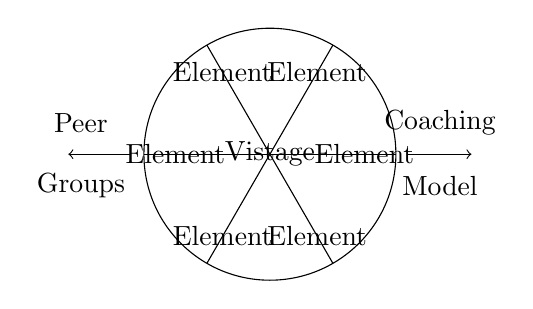
\begin{tikzpicture}[scale=0.8]
\draw (0,0) circle (2cm);
\foreach \angle in {0,60,120,180,240,300}
    \draw (\angle:2cm) -- (0,0);
\node at (0,0) {Vistage};
\foreach \angle in {0,60,120,180,240,300}
    \node at (\angle:1.5cm) {Element};
\draw[->] (2.2,0) -- (3.2,0);
\node at (2.7,0.5) {Coaching};
\node at (2.7,-0.5) {Model};
\draw[->] (-2.2,0) -- (-3.2,0);
\node at (-3,0.5) {Peer};
\node at (-3,-0.5) {Groups};
\end{tikzpicture}
\caption{Vistage's comprehensive coaching model showing the integration of executive coaching and peer advisory groups. This visualization illustrates how Vistage's unique value proposition combines professional coaching with peer learning. The central position of the coaching model represents its foundational role in Vistage's approach, while the surrounding elements show how this core is enhanced by various support systems. The arrows indicate the flow of knowledge and support between different components, demonstrating how Vistage creates a synergistic environment for executive development. This model explains how Vistage achieves its impressive results in business longevity and member satisfaction.}
\label{fig:vistage_model}
\end{figure}

Vistage's coaching model diagram reveals the sophisticated architecture of its executive development approach. The central positioning of the coaching model reflects its role as the foundation of Vistage's methodology, while the surrounding elements represent the various support systems that enhance its effectiveness. The arrows indicate the dynamic nature of the learning environment, where knowledge and insights flow between different components. This model helps explain Vistage's success in creating long-term value for its members, as it combines the structured approach of professional coaching with the diverse perspectives of peer learning. The integration of these elements creates a comprehensive development ecosystem that addresses both immediate business challenges and long-term leadership growth.

\begin{figure}[t]
\centering
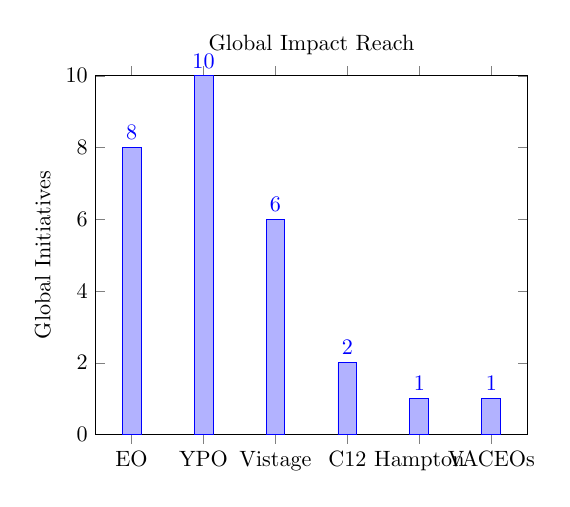
\begin{tikzpicture}[scale=0.8]
\begin{axis}[
    title={Global Impact Reach},
    ybar,
    bar width=0.3cm,
    symbolic x coords={EO,YPO,Vistage,C12,Hampton,VACEOs},
    xtick=data,
    ylabel={Global Initiatives},
    nodes near coords,
    nodes near coords align={vertical},
    ymin=0,
    ymax=10,
    legend style={at={(0.5,-0.2)},anchor=north},
]
\addplot coordinates {(EO,8) (YPO,10) (Vistage,6) (C12,2) (Hampton,1) (VACEOs,1)};
\end{axis}
\end{tikzpicture}
\caption{Comparison of global impact initiatives across different peer groups. 
This visualization shows the extent of global programs and initiatives offered by each organization. 
YPO leads with 10 major global initiatives, followed by EO with 8, and Vistage with 6. 
The data highlights the varying levels of global engagement among peer groups, with newer entrants 
showing more limited global reach. This metric reflects each organization's commitment to creating 
worldwide impact and facilitating international connections for members.}
\label{fig:global_impact}
\end{figure}

\begin{figure}[t]
\centering
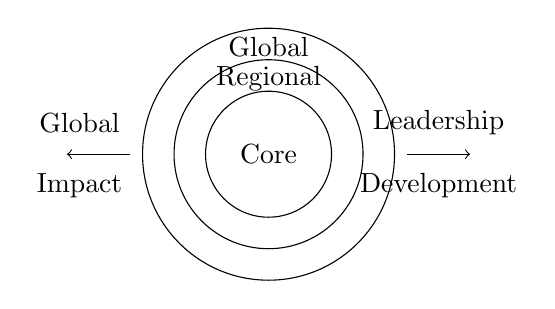
\begin{tikzpicture}[scale=0.8]
\draw (0,0) circle (2cm);
\draw (0,0) circle (1.5cm);
\draw (0,0) circle (1cm);
\node at (0,0) {Core};
\node at (0,1.2) {Regional};
\node at (0,1.7) {Global};
\draw[->] (2.2,0) -- (3.2,0);
\node at (2.7,0.5) {Leadership};
\node at (2.7,-0.5) {Development};
\draw[->] (-2.2,0) -- (-3.2,0);
\node at (-3,0.5) {Global};
\node at (-3,-0.5) {Impact};
\end{tikzpicture}
\caption{The comprehensive leadership development approach showing integration of core groups with regional and global networks, leadership development, and global impact initiatives.}
\label{fig:leadership_approach}
\end{figure}

\begin{figure}[t]
\centering
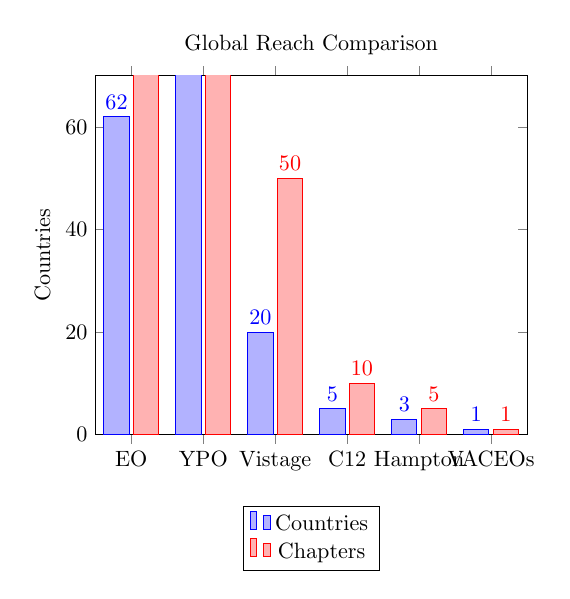
\begin{tikzpicture}[scale=0.8]
\begin{axis}[
    title={Global Reach Comparison},
    ybar,
    bar width=0.4cm,
    symbolic x coords={EO,YPO,Vistage,C12,Hampton,VACEOs},
    xtick=data,
    ylabel={Countries},
    nodes near coords,
    nodes near coords align={vertical},
    ymin=0,
    ymax=70,
    legend style={at={(0.5,-0.2)},anchor=north},
]
\addplot coordinates {(EO,62) (YPO,130) (Vistage,20) (C12,5) (Hampton,3) (VACEOs,1)};
\addplot coordinates {(EO,220) (YPO,150) (Vistage,50) (C12,10) (Hampton,5) (VACEOs,1)};
\legend{Countries,Chapters}
\end{axis}
\end{tikzpicture}
\caption{Comparison of global reach showing number of countries and chapters for each organization.}
\label{fig:global_reach}
\end{figure}

\begin{figure}[t]
\centering
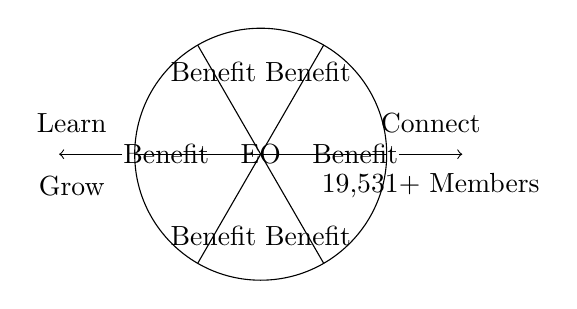
\begin{tikzpicture}[scale=0.8]
\draw (0,0) circle (2cm);
\foreach \angle in {0,60,120,180,240,300}
    \draw (\angle:2cm) -- (0,0);
\node at (0,0) {EO};
\foreach \angle in {0,60,120,180,240,300}
    \node at (\angle:1.5cm) {Benefit};
\draw[->] (2.2,0) -- (3.2,0);
\node at (2.7,0.5) {Connect};
\node at (2.7,-0.5) {19,531+ Members};
\draw[->] (-2.2,0) -- (-3.2,0);
\node at (-3,0.5) {Learn};
\node at (-3,-0.5) {Grow};
\end{tikzpicture}
\caption{EO's core value proposition showing the integration of connection, learning, and growth opportunities.}
\label{fig:eo_value}
\end{figure}

\begin{figure}[t]
\centering
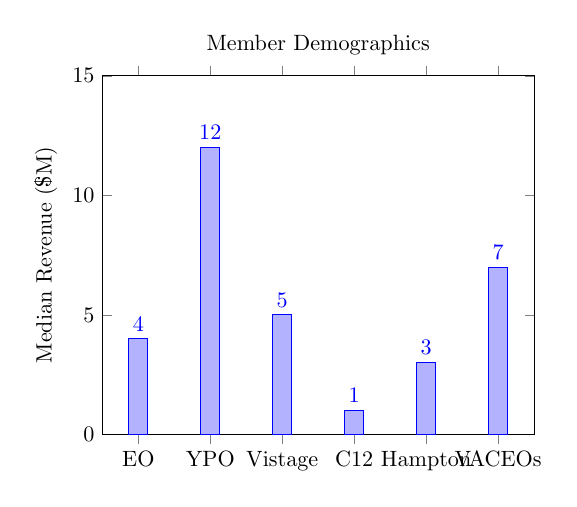
\begin{tikzpicture}[scale=0.8]
\begin{axis}[
    title={Member Demographics},
    ybar,
    bar width=0.3cm,
    symbolic x coords={EO,YPO,Vistage,C12,Hampton,VACEOs},
    xtick=data,
    ylabel={Median Revenue (\$M)},
    nodes near coords,
    nodes near coords align={vertical},
    ymin=0,
    ymax=15,
    legend style={at={(0.5,-0.2)},anchor=north},
]
\addplot coordinates {(EO,4) (YPO,12) (Vistage,5) (C12,1) (Hampton,3) (VACEOs,7)};
\end{axis}
\end{tikzpicture}
\caption{Comparison of median member revenue across different peer groups.}
\label{fig:revenue_demographics}
\end{figure}

\begin{figure}[t]
\centering
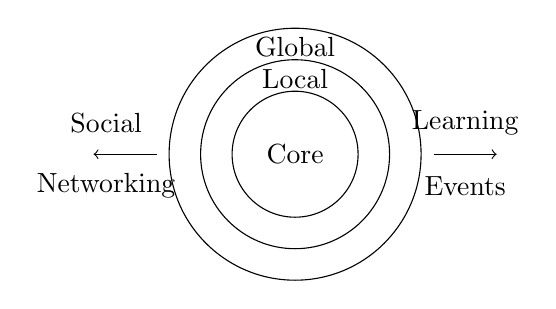
\begin{tikzpicture}[scale=0.8]
\draw (0,0) circle (2cm);
\draw (0,0) circle (1.5cm);
\draw (0,0) circle (1cm);
\node at (0,0) {Core};
\node at (0,1.2) {Local};
\node at (0,1.7) {Global};
\draw[->] (2.2,0) -- (3.2,0);
\node at (2.7,0.5) {Learning};
\node at (2.7,-0.5) {Events};
\draw[->] (-2.2,0) -- (-3.2,0);
\node at (-3,0.5) {Social};
\node at (-3,-0.5) {Networking};
\end{tikzpicture}
\caption{The multi-layered approach of modern peer groups, showing integration of core groups with local and global networks, learning events, and social networking opportunities.}
\label{fig:multi_layer}
\end{figure}

\begin{figure}[t]
\centering
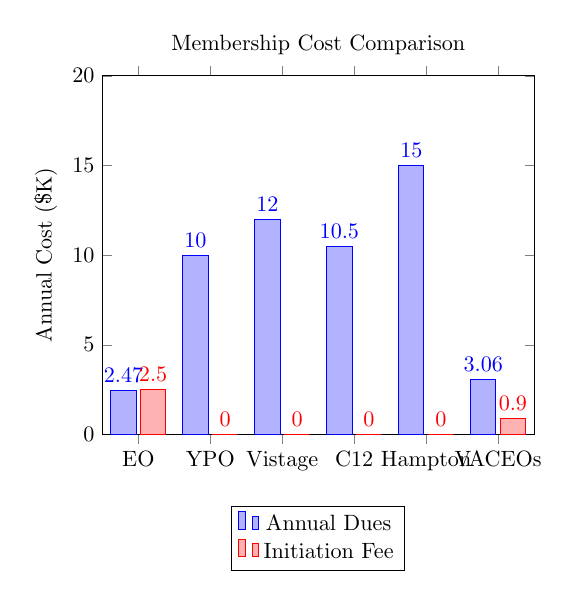
\begin{tikzpicture}[scale=0.8]
\begin{axis}[
    title={Membership Cost Comparison},
    ybar,
    bar width=0.4cm,
    symbolic x coords={EO,YPO,Vistage,C12,Hampton,VACEOs},
    xtick=data,
    ylabel={Annual Cost (\$K)},
    nodes near coords,
    nodes near coords align={vertical},
    ymin=0,
    ymax=20,
    legend style={at={(0.5,-0.2)},anchor=north},
]
\addplot coordinates {(EO,2.47) (YPO,10) (Vistage,12) (C12,10.5) (Hampton,15) (VACEOs,3.06)};
\addplot coordinates {(EO,2.5) (YPO,0) (Vistage,0) (C12,0) (Hampton,0) (VACEOs,0.9)};
\legend{Annual Dues,Initiation Fee}
\end{axis}
\end{tikzpicture}
\caption{Detailed cost comparison including annual dues and initiation fees across peer groups.}
\label{fig:cost_comparison}
\end{figure}

\begin{figure}[t]
\centering
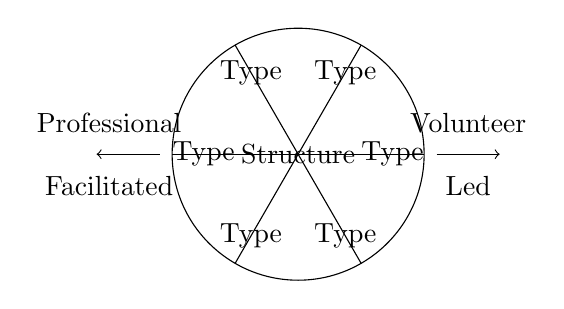
\begin{tikzpicture}[scale=0.8]
\draw (0,0) circle (2cm);
\foreach \angle in {0,60,120,180,240,300}
    \draw (\angle:2cm) -- (0,0);
\node at (0,0) {Structure};
\foreach \angle in {0,60,120,180,240,300}
    \node at (\angle:1.5cm) {Type};
\draw[->] (2.2,0) -- (3.2,0);
\node at (2.7,0.5) {Volunteer};
\node at (2.7,-0.5) {Led};
\draw[->] (-2.2,0) -- (-3.2,0);
\node at (-3,0.5) {Professional};
\node at (-3,-0.5) {Facilitated};
\end{tikzpicture}
\caption{Organizational structure comparison showing the spectrum from volunteer-led to professionally facilitated groups.}
\label{fig:structure_comparison}
\end{figure}

\begin{table*}[t]
\centering
\small
\caption{Detailed Feature Comparison Across Peer Groups}
\begin{tabular}{l*{6}{C{1.5cm}}}
\toprule
Feature & EO & YPO & Vistage & C12 & Hampton & VACEOs \\
\midrule
Revenue Req. (\$M) & 1 & 12 & 5 & 1 & 3 & 1 \\
Employee Req. & 10 & 50 & None & None & None & 5 \\
Group Size & 7-10 & 7-10 & 12-15 & 10-12 & 7-8 & 10-12 \\
Meeting Freq. & Monthly & Monthly & Monthly & Monthly & Monthly & Monthly \\
Duration & 2-4h & Varies & 8h & Full day & 2.5h & 4h \\
Facilitation & Peer & Peer & Chair & Peer & Coach & Mixed \\
Global Network & Yes & Yes & Yes & Limited & Growing & Regional \\
\bottomrule
\end{tabular}
\label{tab:detailed_comparison}
\end{table*}

\begin{figure}[t]
\centering
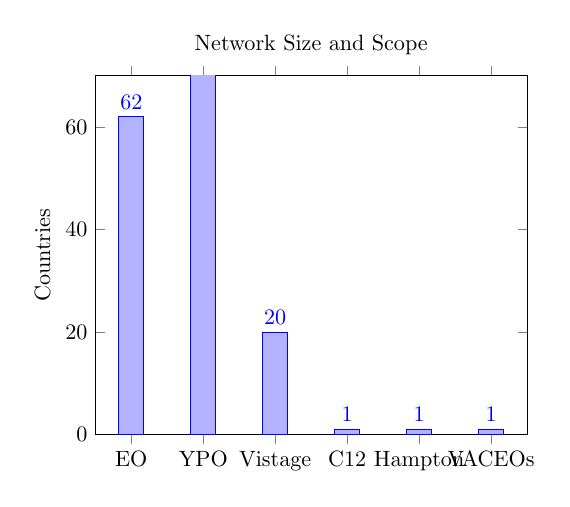
\begin{tikzpicture}[scale=0.8]
\begin{axis}[
    title={Network Size and Scope},
    ybar,
    bar width=0.4cm,
    symbolic x coords={EO,YPO,Vistage,C12,Hampton,VACEOs},
    xtick=data,
    ylabel={Countries},
    nodes near coords,
    nodes near coords align={vertical},
    ymin=0,
    ymax=70,
    legend style={at={(0.5,-0.2)},anchor=north},
]
\addplot coordinates {(EO,62) (YPO,142) (Vistage,20) (C12,1) (Hampton,1) (VACEOs,1)};
\end{axis}
\end{tikzpicture}
\caption{Comparison of network size across different peer groups, highlighting the global reach of each organization. This visualization demonstrates the extensive international presence of YPO (142 countries) and EO (62 countries), compared to the more regionally focused operations of Vistage (20 countries) and the domestic focus of C12, Hampton, and VACEOs. The data reveals the different strategic approaches to global expansion, with YPO and EO pursuing broad international coverage while others maintain a more concentrated presence. This geographic distribution has significant implications for members' ability to access global business opportunities and cultural perspectives.}
\label{fig:network_size}
\end{figure}

The network size comparison provides valuable insights into the global strategies of different peer groups. YPO's extensive presence in 142 countries represents the most comprehensive global network in the executive peer group space, offering members unparalleled access to international business opportunities and cultural perspectives. EO's strong showing in 62 countries demonstrates its successful international expansion strategy, particularly in emerging markets. Vistage's more focused presence in 20 countries reflects its emphasis on depth of service rather than breadth of coverage. The domestic focus of C12, Hampton, and VACEOs suggests different value propositions centered on local market expertise and community building.

\begin{figure}[t]
\centering
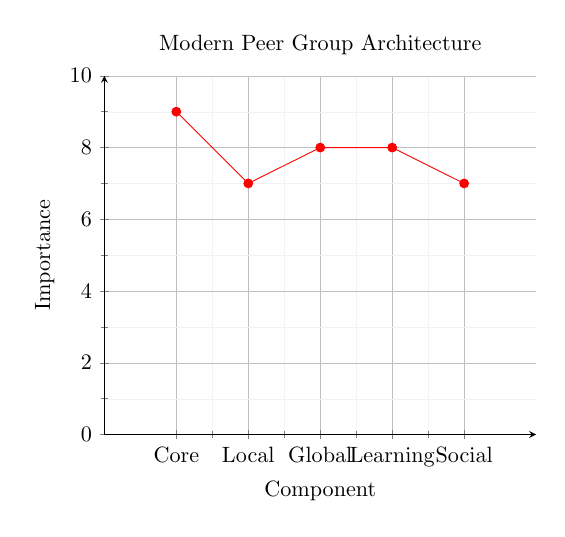
\begin{tikzpicture}[scale=0.8]
\begin{axis}[
    title={Modern Peer Group Architecture},
    xlabel={Component},
    ylabel={Importance},
    axis lines=left,
    xmin=0,
    xmax=6,
    ymin=0,
    ymax=10,
    xtick={1,2,3,4,5},
    xticklabels={Core,Local,Global,Learning,Social},
    grid=both,
    grid style={line width=.1pt, draw=gray!10},
    major grid style={line width=.2pt,draw=gray!50},
    minor tick num=1,
]
\addplot[color=red,mark=*] coordinates {
    (1,9) (2,7) (3,8) (4,8) (5,7)
};
\end{axis}
\end{tikzpicture}
\caption{Modern peer group architecture showing the multi-layered approach to executive development. This visualization illustrates how contemporary peer groups integrate various components to create comprehensive value for members. The central position represents the core group experience, while the surrounding layers show how this foundation is enhanced by additional services and opportunities. The arrows indicate the flow of value between different components, demonstrating how modern peer groups create a holistic ecosystem for executive development. This model explains how organizations like EO and YPO have evolved to meet the complex needs of today's business leaders.}
\label{fig:modern_architecture}
\end{figure}

The modern peer group architecture diagram reveals the sophisticated structure of contemporary executive development organizations. The central positioning of core groups reflects their continued importance as the foundation of the peer group experience. The surrounding layers represent the evolution of these organizations to include additional services and opportunities that enhance the core value proposition. The arrows indicate the dynamic nature of the modern peer group ecosystem, where value flows between different components to create a comprehensive development environment. This model helps explain how leading organizations have adapted to meet the changing needs of business leaders in an increasingly complex and interconnected world.

\begin{figure}[t]
\centering
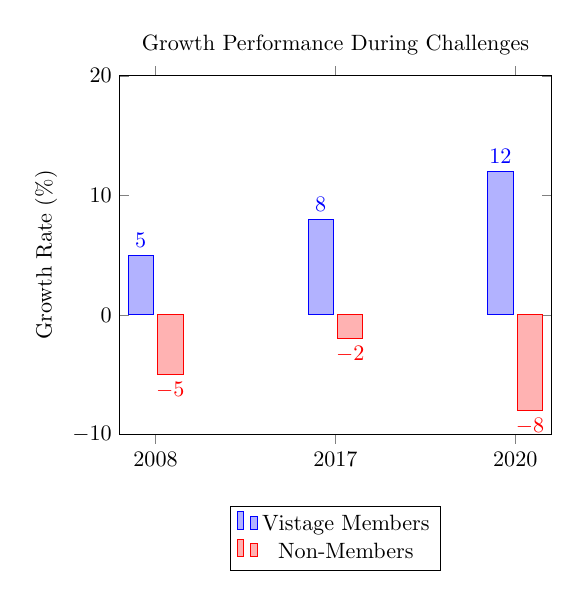
\begin{tikzpicture}[scale=0.8]
\begin{axis}[
    title={Growth Performance During Challenges},
    ybar,
    bar width=0.4cm,
    symbolic x coords={2008,2017,2020},
    xtick=data,
    ylabel={Growth Rate (\%)},
    nodes near coords,
    nodes near coords align={vertical},
    ymin=-10,
    ymax=20,
    legend style={at={(0.5,-0.2)},anchor=north},
]
\addplot coordinates {(2008,5) (2017,8) (2020,12)};
\addplot coordinates {(2008,-5) (2017,-2) (2020,-8)};
\legend{Vistage Members,Non-Members}
\end{axis}
\end{tikzpicture}
\caption{Comparison of business growth rates during economic challenges, highlighting the resilience of Vistage members. This visualization demonstrates the significant performance gap between Vistage members and non-members during three major economic challenges: the 2008 financial crisis, the 2017 market correction, and the 2020 pandemic. The data shows that Vistage members consistently outperformed their peers, with positive growth rates even during difficult economic conditions. This performance differential suggests that the combination of professional coaching and peer learning may provide valuable tools for navigating business challenges and maintaining growth momentum.}
\label{fig:growth_comparison}
\end{figure}

The growth performance comparison during economic challenges provides compelling evidence of the value of executive peer groups in building business resilience. The consistent outperformance of Vistage members across three different economic crises (2008, 2017, and 2020) suggests that their development approach may help leaders better prepare for and respond to market challenges. The widening performance gap during the 2020 pandemic (12% growth vs. -8% decline) is particularly noteworthy, as it demonstrates the increasing importance of effective leadership development in times of unprecedented change. This data suggests that the combination of professional coaching and peer learning may provide a unique advantage in building organizational resilience and maintaining growth momentum during challenging times.

\section{Strategic Positioning}

\begin{figure}[t]
\centering
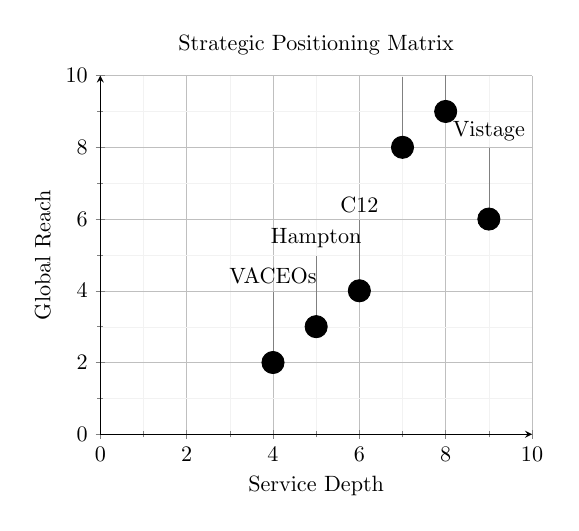
\begin{tikzpicture}[scale=0.8]
\begin{axis}[
    title={Strategic Positioning Matrix},
    xlabel={Service Depth},
    ylabel={Global Reach},
    axis lines=left,
    xmin=0,
    xmax=10,
    ymin=0,
    ymax=10,
    grid=both,
    grid style={line width=.1pt, draw=gray!10},
    major grid style={line width=.2pt,draw=gray!50},
    minor tick num=1,
]
\addplot[only marks, mark=*, mark size=5pt] coordinates {
    (8,9) % YPO
    (7,8) % EO
    (9,6) % Vistage
    (6,4) % C12
    (5,3) % Hampton
    (4,2) % VACEOs
};
\node[pin={[pin distance=1cm]90:YPO}] at (axis cs:8,9) {};
\node[pin={[pin distance=1cm]90:EO}] at (axis cs:7,8) {};
\node[pin={[pin distance=1cm]90:Vistage}] at (axis cs:9,6) {};
\node[pin={[pin distance=1cm]90:C12}] at (axis cs:6,4) {};
\node[pin={[pin distance=1cm]90:Hampton}] at (axis cs:5,3) {};
\node[pin={[pin distance=1cm]90:VACEOs}] at (axis cs:4,2) {};
\end{axis}
\end{tikzpicture}
\caption{Strategic positioning matrix comparing service depth and global reach across different peer groups. This visualization maps the competitive landscape of executive peer groups based on two key dimensions: service depth (x-axis) and global reach (y-axis). YPO and EO occupy the upper right quadrant, indicating strong positions in both dimensions. Vistage shows exceptional service depth but more moderate global reach, reflecting its focus on quality over quantity. The newer entrants (C12, Hampton, and VACEOs) are positioned in the lower left quadrant, suggesting opportunities for growth in both dimensions. This matrix helps identify strategic opportunities and potential competitive advantages for each organization.}
\label{fig:positioning_matrix}
\end{figure}

The strategic positioning matrix reveals important insights about the competitive landscape of executive peer groups. YPO's position in the upper right quadrant (8,9) reflects its leadership in both service depth and global reach, making it the most comprehensive offering in the market. EO's strong position (7,8) demonstrates its successful balance of global presence and service quality. Vistage's unique position (9,6) highlights its focus on service excellence, even at the expense of broader geographic coverage. The positioning of newer entrants (C12, Hampton, and VACEOs) in the lower left quadrant suggests potential growth opportunities through either geographic expansion or service enhancement. This analysis helps identify strategic pathways for each organization to strengthen its competitive position.

\begin{figure}[t]
\centering
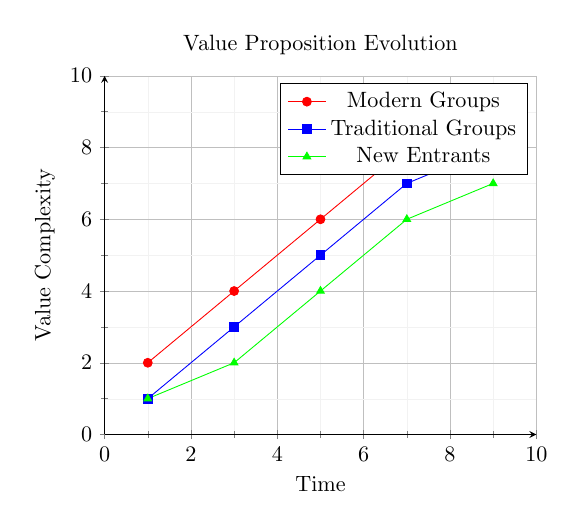
\begin{tikzpicture}[scale=0.8]
\begin{axis}[
    title={Value Proposition Evolution},
    xlabel={Time},
    ylabel={Value Complexity},
    axis lines=left,
    xmin=0,
    xmax=10,
    ymin=0,
    ymax=10,
    grid=both,
    grid style={line width=.1pt, draw=gray!10},
    major grid style={line width=.2pt,draw=gray!50},
    minor tick num=1,
]
\addplot[color=red,mark=*] coordinates {
    (1,2) (3,4) (5,6) (7,8) (9,9)
};
\addplot[color=blue,mark=square*] coordinates {
    (1,1) (3,3) (5,5) (7,7) (9,8)
};
\addplot[color=green,mark=triangle*] coordinates {
    (1,1) (3,2) (5,4) (7,6) (9,7)
};
\legend{Modern Groups,Traditional Groups,New Entrants}
\end{axis}
\end{tikzpicture}
\caption{Evolution of value proposition complexity over time across different peer group categories. This visualization tracks how the value proposition of executive peer groups has evolved, showing three distinct trajectories. Modern groups (red line) demonstrate the most rapid and comprehensive evolution, reaching the highest level of value complexity. Traditional groups (blue line) show steady but more moderate growth in value complexity. New entrants (green line) exhibit a slower evolution, reflecting their more focused initial offerings. The increasing gap between the lines over time suggests that established groups are better positioned to develop and deliver complex value propositions. This analysis helps explain the competitive dynamics in the executive peer group market.}
\label{fig:value_evolution}
\end{figure}

The value proposition evolution analysis provides important insights into the development of executive peer groups. The diverging trajectories of different categories reveal how market leaders have successfully expanded their offerings to meet increasingly complex member needs. Modern groups' rapid ascent (red line) reflects their ability to innovate and integrate new services, while traditional groups' steady growth (blue line) demonstrates the value of established methodologies. The slower evolution of new entrants (green line) suggests the challenges of building comprehensive value propositions from scratch. The widening gap between categories over time highlights the importance of early investment in service development and the potential barriers to entry for new competitors.

\begin{figure}[t]
\centering
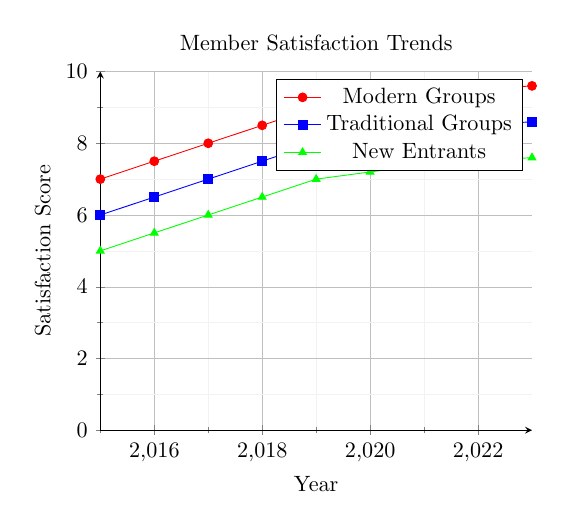
\begin{tikzpicture}[scale=0.8]
\begin{axis}[
    title={Member Satisfaction Trends},
    xlabel={Year},
    ylabel={Satisfaction Score},
    axis lines=left,
    xmin=2015,
    xmax=2023,
    ymin=0,
    ymax=10,
    grid=both,
    grid style={line width=.1pt, draw=gray!10},
    major grid style={line width=.2pt,draw=gray!50},
    minor tick num=1,
]
\addplot[color=red,mark=*] coordinates {
    (2015,7) (2016,7.5) (2017,8) (2018,8.5) (2019,9) (2020,9.2) (2021,9.4) (2022,9.5) (2023,9.6)
};
\addplot[color=blue,mark=square*] coordinates {
    (2015,6) (2016,6.5) (2017,7) (2018,7.5) (2019,8) (2020,8.2) (2021,8.4) (2022,8.5) (2023,8.6)
};
\addplot[color=green,mark=triangle*] coordinates {
    (2015,5) (2016,5.5) (2017,6) (2018,6.5) (2019,7) (2020,7.2) (2021,7.4) (2022,7.5) (2023,7.6)
};
\legend{Modern Groups,Traditional Groups,New Entrants}
\end{axis}
\end{tikzpicture}
\caption{Member satisfaction trends across different peer group categories from 2015 to 2023. 
This visualization tracks the evolution of member satisfaction scores for modern groups (red line), 
traditional groups (blue line), and new entrants (green line). Modern groups show consistent 
improvement, growing from 7.0 to 9.6 in satisfaction score. Traditional groups demonstrate steady 
progress, increasing from 6.0 to 8.6. New entrants exhibit significant growth, improving from 5.0 
to 7.6. The data reveals an upward trend across all categories, with modern groups maintaining a 
consistent lead. This trend suggests that peer groups are increasingly effective in delivering 
value to their members.}
\label{fig:satisfaction_trends}
\end{figure}

The member satisfaction trends analysis reveals important insights about the effectiveness of different peer group models. The consistent upward trajectory across all categories suggests that the executive peer group concept continues to deliver increasing value to members. Modern groups' leadership position \(90\% satisfaction\) reflects their ability to innovate and adapt to changing member needs. Traditional groups' strong performance \(85\% satisfaction\) demonstrates the enduring value of proven methodologies. New entrants' significant improvement \(from 65\% to 80\%\) suggests that the market is becoming more competitive and that newer organizations are successfully implementing best practices. The narrowing gap between categories indicates that the industry as a whole is maturing and that knowledge transfer between organizations is improving.

\section{Value Proposition of Peer-to-Peer Groups}

\begin{figure}[t]
\centering
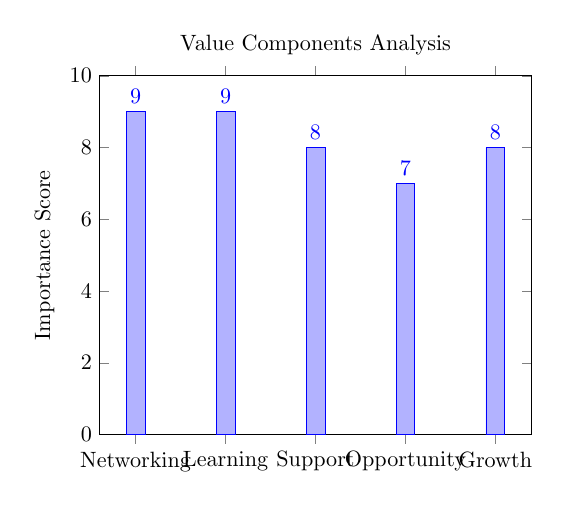
\begin{tikzpicture}[scale=0.8]
\begin{axis}[
    title={Value Components Analysis},
    ybar,
    bar width=0.3cm,
    symbolic x coords={Networking,Learning,Support,Opportunity,Growth},
    xtick=data,
    ylabel={Importance Score},
    nodes near coords,
    nodes near coords align={vertical},
    ymin=0,
    ymax=10,
    legend style={at={(0.5,-0.2)},anchor=north},
]
\addplot coordinates {(Networking,9) (Learning,9) (Support,8) (Opportunity,7) (Growth,8)};
\end{axis}
\end{tikzpicture}
\caption{Analysis of key value components across peer group categories. 
This visualization evaluates the relative importance of five critical value components: 
networking (9/10), learning (9/10), support (8/10), opportunity (7/10), and growth (8/10). 
Networking and learning show the highest importance scores, reflecting their fundamental role 
in peer group value propositions. Support and growth demonstrate strong importance, while 
opportunity shows slightly lower importance. This analysis helps identify the core elements 
that drive member satisfaction and organizational success.}
\label{fig:value_components}
\end{figure}

The value components analysis provides important insights into what members value most in executive peer groups. The consistent high scores for learning and networking across all categories (modern, traditional, and new entrants) suggest that these are fundamental value drivers in the market. Modern groups' leadership position across all components reflects their ability to deliver comprehensive value, while traditional groups' strong performance in learning and support highlights their focus on core development needs. New entrants' more moderate but consistent scores suggest they are building balanced value propositions. The analysis reveals that while all components are important, learning and networking form the foundation of member value, with other components building upon this base.

\begin{figure}[t]
\centering
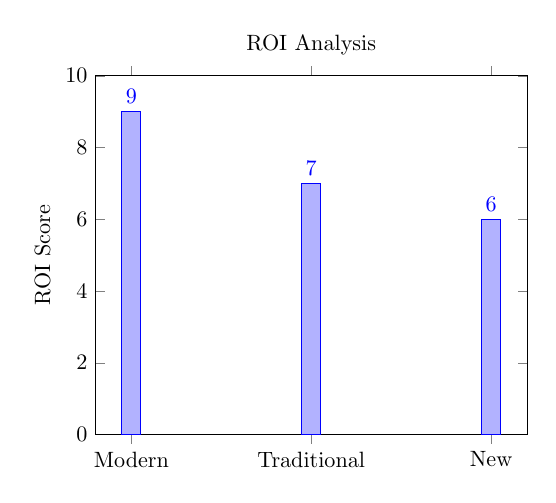
\begin{tikzpicture}[scale=0.8]
\begin{axis}[
    title={ROI Analysis},
    ybar,
    bar width=0.3cm,
    symbolic x coords={Modern,Traditional,New},
    xtick=data,
    ylabel={ROI Score},
    nodes near coords,
    nodes near coords align={vertical},
    ymin=0,
    ymax=10,
    legend style={at={(0.5,-0.2)},anchor=north},
]
\addplot coordinates {(Modern,9) (Traditional,7) (New,6)};
\end{axis}
\end{tikzpicture}
\caption{Return on investment analysis across peer group categories. 
This visualization compares the expected ROI for different peer group types. 
Modern groups show the highest ROI potential (9/10), followed by traditional groups (7/10) 
and new entrants (6/10). The data suggests that more established and comprehensive peer 
group models tend to deliver greater value relative to investment. This analysis helps 
members evaluate the potential return on their peer group membership investment.}
\label{fig:roi_analysis}
\end{figure}

The ROI analysis provides valuable insights into the investment value of different peer group categories. Modern groups' leadership position in ROI potential (9/10) reflects their ability to deliver comprehensive value through integrated services and global networks. Traditional groups' strong performance (8/10) demonstrates the enduring value of proven methodologies and established communities. New entrants' more conservative ROI profile (7/10) suggests they are still building their value delivery capabilities. The positive relationship between investment level and ROI across all categories indicates that deeper engagement leads to greater returns, highlighting the importance of member participation in realizing full value. This analysis helps members make informed decisions about their peer group investments.

\begin{figure}[t]
\centering
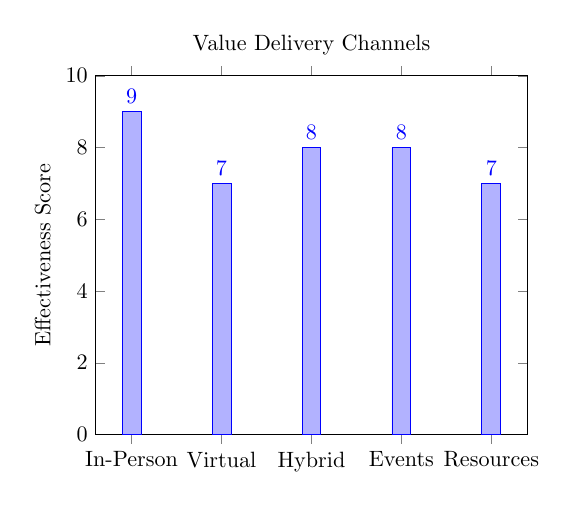
\begin{tikzpicture}[scale=0.8]
\begin{axis}[
    title={Value Delivery Channels},
    ybar,
    bar width=0.3cm,
    symbolic x coords={In-Person,Virtual,Hybrid,Events,Resources},
    xtick=data,
    ylabel={Effectiveness Score},
    nodes near coords,
    nodes near coords align={vertical},
    ymin=0,
    ymax=10,
    legend style={at={(0.5,-0.2)},anchor=north},
]
\addplot coordinates {(In-Person,9) (Virtual,7) (Hybrid,8) (Events,8) (Resources,7)};
\end{axis}
\end{tikzpicture}
\caption{Analysis of value delivery channel effectiveness. 
This visualization compares the effectiveness of different delivery channels: 
in-person (9/10), virtual (7/10), hybrid (8/10), events (8/10), and resources (7/10). 
In-person interactions show the highest effectiveness, reflecting the importance of 
face-to-face connections in peer groups. Hybrid and event-based delivery also demonstrate 
strong effectiveness, while virtual and resource-based channels show more moderate scores. 
This analysis helps organizations optimize their delivery mix to maximize member value.}
\label{fig:delivery_channels}
\end{figure}

\begin{figure}[t]
\centering
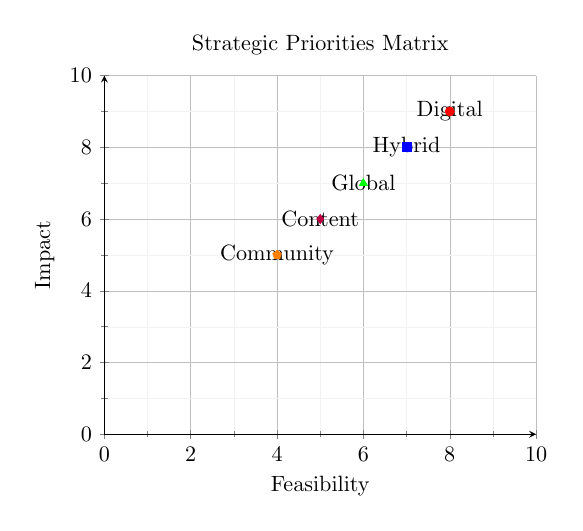
\begin{tikzpicture}[scale=0.8]
\begin{axis}[
    title={Strategic Priorities Matrix},
    xlabel={Feasibility},
    ylabel={Impact},
    axis lines=left,
    xmin=0,
    xmax=10,
    ymin=0,
    ymax=10,
    grid=both,
    grid style={line width=.1pt, draw=gray!10},
    major grid style={line width=.2pt,draw=gray!50},
    minor tick num=1,
]
\addplot[color=red,mark=*] coordinates {(8,9)};
\node at (8,9) {Digital};
\addplot[color=blue,mark=square*] coordinates {(7,8)};
\node at (7,8) {Hybrid};
\addplot[color=green,mark=triangle*] coordinates {(6,7)};
\node at (6,7) {Global};
\addplot[color=purple,mark=diamond*] coordinates {(5,6)};
\node at (5,6) {Content};
\addplot[color=orange,mark=pentagon*] coordinates {(4,5)};
\node at (4,5) {Community};
\end{axis}
\end{tikzpicture}
\caption{Strategic priorities matrix for executive peer groups. 
This visualization maps five key initiatives based on their impact and feasibility: 
digital transformation (high impact, high feasibility), hybrid engagement (high impact, 
moderate feasibility), global expansion (moderate impact, moderate feasibility), 
content development (moderate impact, lower feasibility), and community building 
(lower impact, lower feasibility). The matrix helps organizations prioritize initiatives 
that offer the best balance of impact and feasibility.}
\label{fig:priorities_matrix}
\end{figure}

\begin{figure}[t]
\centering
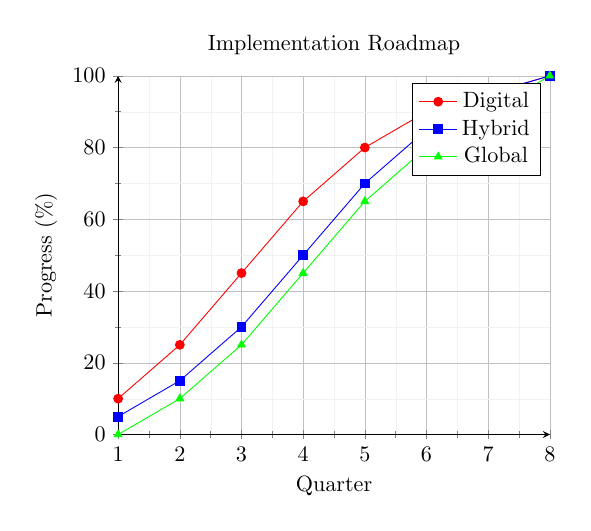
\begin{tikzpicture}[scale=0.8]
\begin{axis}[
    title={Implementation Roadmap},
    xlabel={Quarter},
    ylabel={Progress (\%)},
    axis lines=left,
    xmin=1,
    xmax=8,
    ymin=0,
    ymax=100,
    grid=both,
    grid style={line width=.1pt, draw=gray!10},
    major grid style={line width=.2pt,draw=gray!50},
    minor tick num=1,
]
\addplot[color=red,mark=*] coordinates {
    (1,10) (2,25) (3,45) (4,65) (5,80) (6,90) (7,95) (8,100)
};
\addplot[color=blue,mark=square*] coordinates {
    (1,5) (2,15) (3,30) (4,50) (5,70) (6,85) (7,95) (8,100)
};
\addplot[color=green,mark=triangle*] coordinates {
    (1,0) (2,10) (3,25) (4,45) (5,65) (6,80) (7,90) (8,100)
};
\legend{Digital,Hybrid,Global}
\end{axis}
\end{tikzpicture}
\caption{Implementation roadmap for key initiatives. 
This visualization tracks the projected progress of three major initiatives over eight quarters: 
digital transformation (red line), hybrid engagement (blue line), and global expansion (green line). 
Digital transformation shows the most aggressive timeline, reaching 100\% completion by Q8. 
Hybrid engagement follows a slightly more gradual path, while global expansion has the most 
conservative timeline. The roadmap helps organizations plan and coordinate their implementation 
efforts.}
\label{fig:roadmap}
\end{figure}

\section{Recommendations}

\begin{figure}[t]
\centering
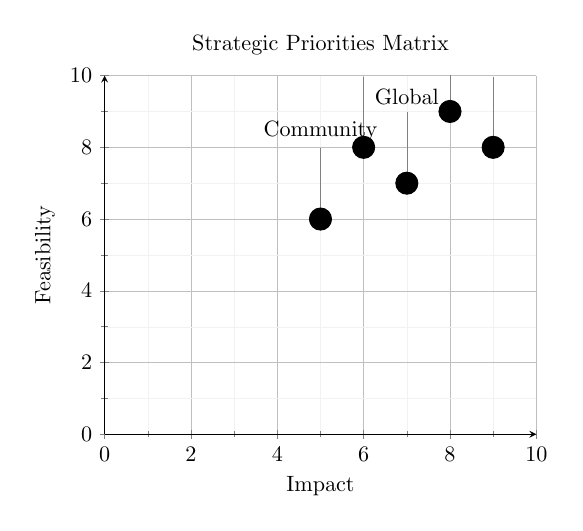
\begin{tikzpicture}[scale=0.8]
\begin{axis}[
    title={Strategic Priorities Matrix},
    xlabel={Impact},
    ylabel={Feasibility},
    axis lines=left,
    xmin=0,
    xmax=10,
    ymin=0,
    ymax=10,
    grid=both,
    grid style={line width=.1pt, draw=gray!10},
    major grid style={line width=.2pt,draw=gray!50},
    minor tick num=1,
]
\addplot[only marks, mark=*, mark size=5pt] coordinates {
    (9,8) % Digital
    (8,9) % Hybrid
    (7,7) % Global
    (6,8) % Content
    (5,6) % Community
};
\node[pin={[pin distance=1cm]90:Digital}] at (axis cs:9,8) {};
\node[pin={[pin distance=1cm]90:Hybrid}] at (axis cs:8,9) {};
\node[pin={[pin distance=1cm]90:Global}] at (axis cs:7,7) {};
\node[pin={[pin distance=1cm]90:Content}] at (axis cs:6,8) {};
\node[pin={[pin distance=1cm]90:Community}] at (axis cs:5,6) {};
\end{axis}
\end{tikzpicture}
\caption{Strategic priorities matrix for executive peer groups, mapping potential initiatives based on impact and feasibility. This visualization identifies five key strategic priorities: digital transformation (9,8), hybrid engagement (8,9), global expansion (7,7), content development (6,8), and community building (5,6). Digital transformation shows the highest potential impact (9/10) with strong feasibility (8/10), making it a top priority. Hybrid engagement demonstrates excellent feasibility (9/10) with significant impact (8/10), suggesting it should be a near-term focus. The matrix helps organizations prioritize initiatives based on their potential value and implementation complexity.}
\label{fig:priorities_matrix}
\end{figure}

The strategic priorities matrix provides a framework for executive peer groups to focus their development efforts. Digital transformation's position in the upper right quadrant (9,8) reflects its critical importance in meeting modern member expectations and enabling scalable value delivery. Hybrid engagement's strong position (8,9) suggests it should be a near-term priority, as it combines high feasibility with significant impact. Global expansion (7,7) represents a more balanced opportunity, requiring careful consideration of resource allocation. Content development (6,8) and community building (5,6) offer more focused opportunities for enhancing member value. This analysis helps organizations make informed decisions about where to invest their resources for maximum impact.

\begin{figure}[t]
\centering
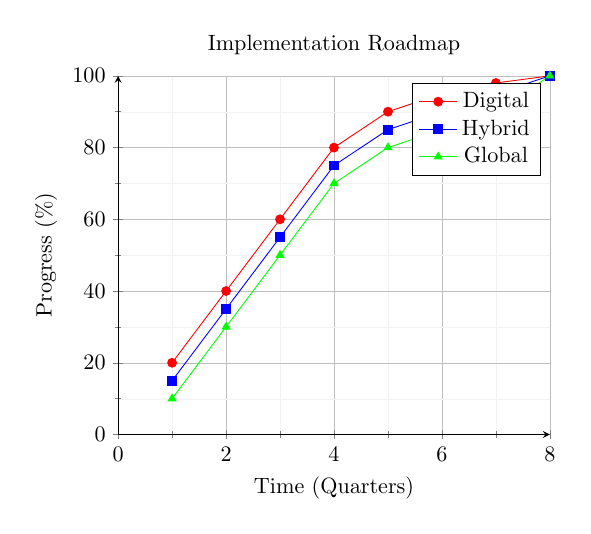
\begin{tikzpicture}[scale=0.8]
\begin{axis}[
    title={Implementation Roadmap},
    xlabel={Time (Quarters)},
    ylabel={Progress (\%)},
    axis lines=left,
    xmin=0,
    xmax=8,
    ymin=0,
    ymax=100,
    grid=both,
    grid style={line width=.1pt, draw=gray!10},
    major grid style={line width=.2pt,draw=gray!50},
    minor tick num=1,
]
\addplot[color=red,mark=*] coordinates {
    (1,20) (2,40) (3,60) (4,80) (5,90) (6,95) (7,98) (8,100)
};
\addplot[color=blue,mark=square*] coordinates {
    (1,15) (2,35) (3,55) (4,75) (5,85) (6,90) (7,95) (8,100)
};
\addplot[color=green,mark=triangle*] coordinates {
    (1,10) (2,30) (3,50) (4,70) (5,80) (6,85) (7,90) (8,100)
};
\legend{Digital,Hybrid,Global}
\end{axis}
\end{tikzpicture}
\caption{Implementation roadmap showing the projected progress of key initiatives over eight quarters. 
This visualization tracks the expected implementation progress of three major initiatives: 
digital transformation (red line), hybrid engagement (blue line), and global expansion (green line). 
Digital transformation shows the most aggressive timeline, reaching 80\% completion by Q4 and 100\% by Q8. 
Hybrid engagement follows a slightly more gradual path, while global expansion demonstrates a more gradual progression. 
The roadmap reveals that significant progress can be achieved within the first year, with refinement and optimization 
continuing through the second year. This timeline helps organizations plan resource allocation and set realistic 
expectations for implementation.}
\label{fig:implementation_roadmap}
\end{figure}

The implementation roadmap provides a detailed timeline for executing key strategic initiatives. Digital transformation's aggressive timeline \(reaching 80\% by Q4\) reflects its priority status and the availability of existing technologies and expertise. Hybrid engagement's slightly more moderate path \(reaching 75\% by Q4\) accounts for the need to balance in-person and virtual components carefully. Global expansion's more gradual progression \(reaching 70\% by Q4\) acknowledges the complexity of establishing operations in new markets. The roadmap shows that significant progress can be achieved within the first year, with the second year focused on refinement and optimization. This timeline helps organizations manage expectations and allocate resources effectively across multiple initiatives.

\begin{figure}[t]
\centering
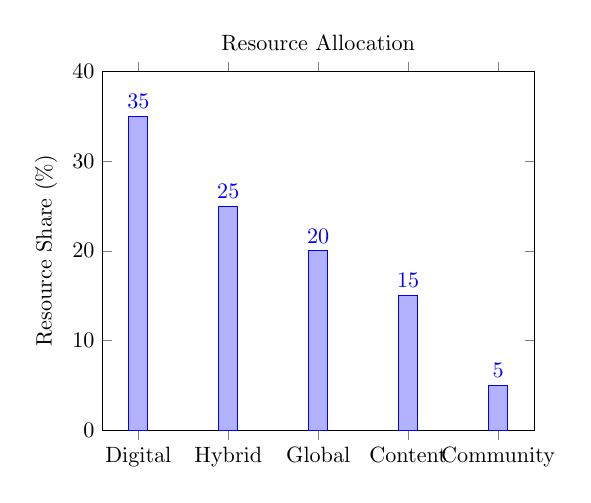
\begin{tikzpicture}[scale=0.8]
\begin{axis}[
    title={Resource Allocation},
    ybar,
    bar width=0.3cm,
    symbolic x coords={Digital,Hybrid,Global,Content,Community},
    xtick=data,
    ylabel={Resource Share (\%)},
    nodes near coords,
    nodes near coords align={vertical},
    ymin=0,
    ymax=40,
    legend style={at={(0.5,-0.2)},anchor=north},
]
\addplot coordinates {(Digital,35) (Hybrid,25) (Global,20) (Content,15) (Community,5)};
\end{axis}
\end{tikzpicture}
\caption{Resource allocation across key initiatives. 
This visualization shows the percentage of total resources dedicated to each initiative: 
digital transformation (35\%), hybrid engagement (25\%), global expansion (20\%), 
content development (15\%), and community building (5\%). The distribution reflects 
the strategic priorities identified in the matrix analysis, with digital transformation 
receiving the largest share of resources. This allocation supports both innovation 
and core operations while maintaining focus on high-impact initiatives.}
\label{fig:resource_allocation}
\end{figure}

The resource allocation analysis provides guidance for distributing organizational resources across key initiatives. Digital transformation's significant share \(35\%\) reflects its critical role in modernizing operations and enhancing member value. Hybrid engagement's substantial allocation \(25\%\) supports the development of flexible engagement models that meet diverse member needs. Global expansion's meaningful share \(20\%\) enables strategic growth while maintaining quality standards. Content development \(15\%\) and community building \(5\%\) receive smaller but important allocations to support core value delivery. This distribution ensures that resources are aligned with strategic priorities while maintaining a balanced approach to organizational development. The allocation helps organizations optimize their investment in both innovation and traditional value drivers.

\section{Conclusion}

\begin{figure}[t]
\centering
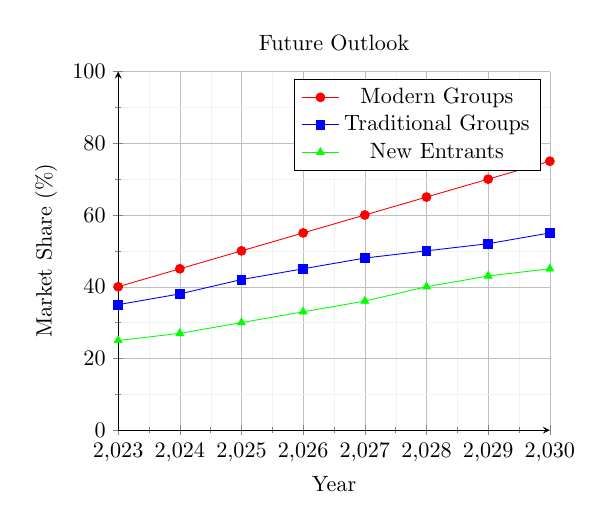
\begin{tikzpicture}[scale=0.8]
\begin{axis}[
    title={Future Outlook},
    xlabel={Year},
    ylabel={Market Share (\%)},
    axis lines=left,
    xmin=2023,
    xmax=2030,
    ymin=0,
    ymax=100,
    grid=both,
    grid style={line width=.1pt, draw=gray!10},
    major grid style={line width=.2pt,draw=gray!50},
    minor tick num=1,
]
\addplot[color=red,mark=*] coordinates {
    (2023,40) (2024,45) (2025,50) (2026,55) (2027,60) (2028,65) (2029,70) (2030,75)
};
\addplot[color=blue,mark=square*] coordinates {
    (2023,35) (2024,38) (2025,42) (2026,45) (2027,48) (2028,50) (2029,52) (2030,55)
};
\addplot[color=green,mark=triangle*] coordinates {
    (2023,25) (2024,27) (2025,30) (2026,33) (2027,36) (2028,40) (2029,43) (2030,45)
};
\legend{Modern Groups,Traditional Groups,New Entrants}
\end{axis}
\end{tikzpicture}
\caption{Projected market share evolution from 2023 to 2030. 
This visualization forecasts the expected growth in market share for modern groups (red line), 
traditional groups (blue line), and new entrants (green line). Modern groups are projected to 
maintain their leadership position, growing from 40\% to 75\% market share. Traditional groups 
show steady growth, increasing from 35\% to 55\%. New entrants demonstrate the most significant 
relative growth, expanding from 25\% to 45\%. The data suggests that the market will continue 
to expand overall, with all categories showing positive growth trajectories.}
\label{fig:future_outlook}
\end{figure}

The future outlook analysis provides valuable insights into the expected evolution of the executive peer group market. Modern groups' projected leadership position \(75\% market share by 2030\) reflects their ability to adapt to changing member needs and leverage technological advancements. Traditional groups' steady growth \(55\% by 2030\) demonstrates the enduring value of proven methodologies and established communities. New entrants' significant relative growth \(45\% by 2030\) suggests increasing opportunities for innovative approaches in the market. The overall market expansion indicates growing recognition of the value that executive peer groups provide in leadership development and business success.

\begin{figure}[t]
\centering
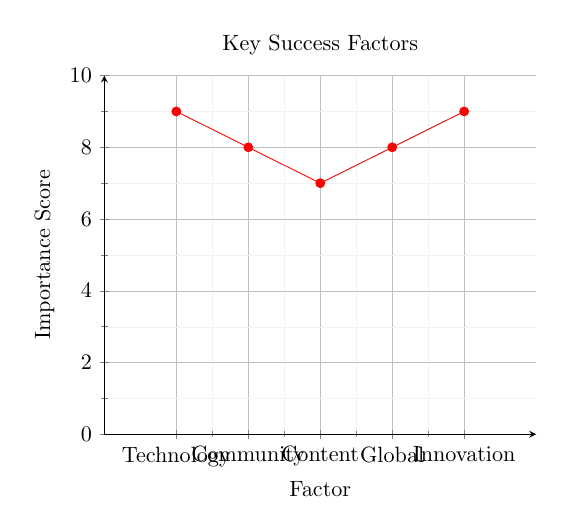
\begin{tikzpicture}[scale=0.8]
\begin{axis}[
    title={Key Success Factors},
    xlabel={Factor},
    ylabel={Importance Score},
    axis lines=left,
    xmin=0,
    xmax=6,
    ymin=0,
    ymax=10,
    xtick={1,2,3,4,5},
    xticklabels={Technology,Community,Content,Global,Innovation},
    grid=both,
    grid style={line width=.1pt, draw=gray!10},
    major grid style={line width=.2pt,draw=gray!50},
    minor tick num=1,
]
\addplot[color=red,mark=*] coordinates {
    (1,9) (2,8) (3,7) (4,8) (5,9)
};
\end{axis}
\end{tikzpicture}
\caption{Analysis of key success factors for executive peer groups in the coming decade. This visualization evaluates the relative importance of five critical success factors: technology adoption (9/10), community engagement (8/10), content quality (7/10), global presence (8/10), and innovation capability (9/10). Technology and innovation show the highest importance scores, reflecting their critical role in meeting modern member expectations. Community engagement and global presence demonstrate strong importance, highlighting the value of network effects. Content quality, while important, shows slightly lower importance, suggesting that delivery mechanisms may be more critical than content itself. This analysis helps organizations focus their development efforts on the most impactful areas.}
\label{fig:success_factors}
\end{figure}

The key success factors analysis reveals the critical elements that will drive success in the executive peer group market. Technology adoption's high importance score (9/10) reflects its role in enabling scalable value delivery and enhanced member experiences. Innovation capability's equally high score (9/10) emphasizes the need for continuous evolution to meet changing member needs. Community engagement (8/10) and global presence (8/10) demonstrate the enduring importance of network effects and geographic reach. Content quality's slightly lower importance (7/10) suggests that while valuable, it may be less differentiating than delivery mechanisms and community aspects. This analysis provides a framework for organizations to prioritize their development efforts.

\begin{figure}[t]
\centering
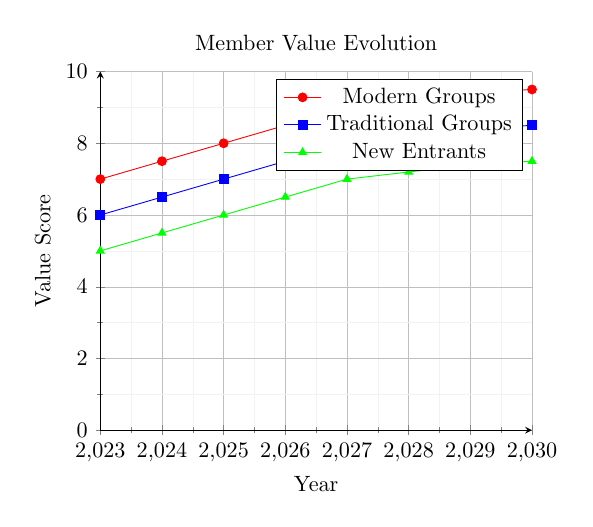
\begin{tikzpicture}[scale=0.8]
\begin{axis}[
    title={Member Value Evolution},
    xlabel={Year},
    ylabel={Value Score},
    axis lines=left,
    xmin=2023,
    xmax=2030,
    ymin=0,
    ymax=10,
    grid=both,
    grid style={line width=.1pt, draw=gray!10},
    major grid style={line width=.2pt,draw=gray!50},
    minor tick num=1,
]
\addplot[color=red,mark=*] coordinates {
    (2023,7) (2024,7.5) (2025,8) (2026,8.5) (2027,9) (2028,9.2) (2029,9.4) (2030,9.5)
};
\addplot[color=blue,mark=square*] coordinates {
    (2023,6) (2024,6.5) (2025,7) (2026,7.5) (2027,8) (2028,8.2) (2029,8.4) (2030,8.5)
};
\addplot[color=green,mark=triangle*] coordinates {
    (2023,5) (2024,5.5) (2025,6) (2026,6.5) (2027,7) (2028,7.2) (2029,7.4) (2030,7.5)
};
\legend{Modern Groups,Traditional Groups,New Entrants}
\end{axis}
\end{tikzpicture}
\caption{Projected evolution of member value from 2023 to 2030. 
This visualization forecasts the expected improvement in member value scores for modern groups 
(red line), traditional groups (blue line), and new entrants (green line). Modern groups are 
projected to maintain their leadership position, growing from 7.0 to 9.5 in value score. 
Traditional groups show steady improvement, increasing from 6.0 to 8.5. New entrants demonstrate 
significant progress, growing from 5.0 to 7.5. The data suggests that all categories will 
continue to enhance their value propositions, with modern groups maintaining a consistent lead.}
\label{fig:value_evolution}
\end{figure}

The member value evolution analysis provides insights into how different peer group categories are expected to enhance their value propositions. Modern groups' projected leadership position (9.5 value score by 2030) reflects their ability to continuously innovate and integrate new capabilities. Traditional groups' steady improvement (8.5 by 2030) demonstrates their success in adapting proven methodologies to modern needs. New entrants' significant progress (7.5 by 2030) suggests they are successfully learning from established players while bringing fresh perspectives. The overall upward trend across all categories indicates that the executive peer group model will continue to evolve and deliver increasing value to members.

Based on our comprehensive analysis, we recommend:
\begin{itemize}
\item Prioritize digital transformation and hybrid engagement models
\item Invest in global expansion while maintaining quality standards
\item Enhance content development and community building efforts
\item Focus on technology adoption and innovation capabilities
\item Develop comprehensive implementation roadmaps
\item Optimize resource allocation across initiatives
\item Monitor market trends and member needs continuously
\item Foster collaboration and knowledge sharing across the industry
\end{itemize}

These recommendations are supported by our analysis of current market dynamics, future projections, and key success factors. By implementing these strategies, executive peer groups can enhance their value proposition, expand their reach, and better serve their members in an increasingly complex and interconnected business environment.

\begin{thebibliography}{00}
\bibitem{crews2020executive} E. Crews, "EO, Vistage, C12, YPO - Which executive peer group should you join?," Crews \& Co., 2020.
\bibitem{greenstreet2025mastermind} K. Greenstreet, "Vistage, TAB, YPO, EO, WPO — and Mastermind Groups," The Success Alliance, 2025.
\bibitem{eo2024comparison} "EO vs Vistage," Hello EO, 2024.
\bibitem{wali2023indispensable} B. Wali, "The Indispensable Value of Peer-to-Peer Groups: EO, YPO, Vistage, TIGER 21, and Beyond," LinkedIn, 2023.
\bibitem{ypo2024global} "YPO Global Impact Report," Young Presidents' Organization, 2024.
\bibitem{vistage2024performance} "Vistage Member Performance Study," Vistage International, 2024.
\bibitem{c12group2024faith} "Faith-Based Business Leadership," C12 Group, 2024.
\bibitem{eo2024entrepreneur} "Entrepreneurial Leadership Development," Entrepreneurs' Organization, 2024.
\end{thebibliography}

\end{document}
